% the manuscript number NODY-D-13-00859R1
% 2013-7-12 Submitted to ND using dkdeng

\input df-headinput-cssp
\begin{filecontents*}{example.eps}
%!PS-Adobe-3.0 EPSF-3.0
%%BoundingBox: 19 19 221 221
%%CreationDate: Mon Sep 29 1997
%%Creator: programmed by hand (JK)
%%EndComments
gsave
newpath
  20 20 moveto
  20 220 lineto
  220 220 lineto
  220 20 lineto
closepath
2 setlinewidth
gsave
  .4 setgray fill
grestore
stroke
grestore
\end{filecontents*}
%
\RequirePackage{fix-cm}
%
%\documentclass{svjour3}                     % onecolumn (standard format)
%\documentclass[smallcondensed]{svjour3}     % onecolumn (ditto)

\documentclass[fleqn,smallextended]{svjour3}       % onecolumn (second format)
%\documentclass[twocolumn]{svjour3}          % twocolumn
%
\usepackage{amsfonts}
\usepackage{mathrsfs}
 \usepackage{amssymb}
 \usepackage{amsmath}
 \usepackage{bm}
 \usepackage[dvips]{color}
%\usepackage{cite}
\allowdisplaybreaks

 \textwidth5.8in
 \textheight9.2in

%
\smartqed  % flush right qed marks, e.g. at end of proof
%
\usepackage{graphicx}
%
% \usepackage{mathptmx}      % use Times fonts if available on your TeX system
%
% insert here the call for the packages your document requires
%\usepackage{latexsym}
% etc.
%
% please place your own definitions here and don't use \def but
% \newcommand{}{}
%
% Insert the name of "your journal" with

\journalname{Nonlinear Dynamics}

\begin{document}

\title{Fault diagnosis of variable pitch for wind turbines based on multi-innovation forgetting gradient identification algorithm
\thanks{This research was supported by Prospective Joint Research Project of Industry, Education and Academy of Jiangsu Province(BY2012071) and China Postdoctoral Science Foundation (2013M531272).}}
% \titlerunning{Newton iterative identification method for input nonlinear systems}
\author{Dinghui Wu \and Yiyang Li} % if too long for running head
\authorrunning{D.H. Wu, Y.Y. Li} % if too long for running head
\institute{D.H. Wu \and Y.Y. Li \at
              Key Laboratory of Advanced Process Control for Light
              Industry (Ministry of Education), Jiangnan University, Wuxi\ 214122, P.R. China\\
 \and
           D.H. Wu (Corresponding author)\at
           Control Science and Engineering Research Center, Jiangnan University, Wuxi\ 214122, P.R. China
%              School of Internet of Things Engineering, Jiangnan University, Wuxi\ 214122, P.R. China
              \\
           \email{wh033098@163.com}
 \and
 }


\date{}
% The correct dates will be entered by the editor

\maketitle


\begin{abstract}

This paper presents the fault diagnosis algorithm of the variable
pitch system for wind turbines. The considered variable pitch
system model is characterized by a second order differential
equation, and is transformed into the discretization equation and
the difference equation. Then the fault diagnosis
problem is transformed into a parameter estimation issue, and the multi-innovation forgetting gradient
(MIFG) identification algorithm is adopted.
As the MIFG algorithm uses not only current data but
also the past data at each iteration, the parameter estimation accuracy can be improved. The validity
of fault diagnosis using MIFG algorithm for pitch system is verified by simulation examples.



 \keywords{Wind turbine \and System identification
\and Pitch system \and Fault diagnosis \and MIFG}
\end{abstract}


\section{Introduction}

Wind energy has contributed to a large part of world power production,
and variable pitch
system has played a important role in wind turbines. Since most wind turbines are located in remote
areas, they are expected to produce energy with reliability and stability \cite{ref:2}.
An effective way to ensure
this is to adopt the advanced fault diagnosis technology, even though it may result in less power
production in some cases \cite{ref:3}.

\begin{figure}[!htb]
  %\centering
  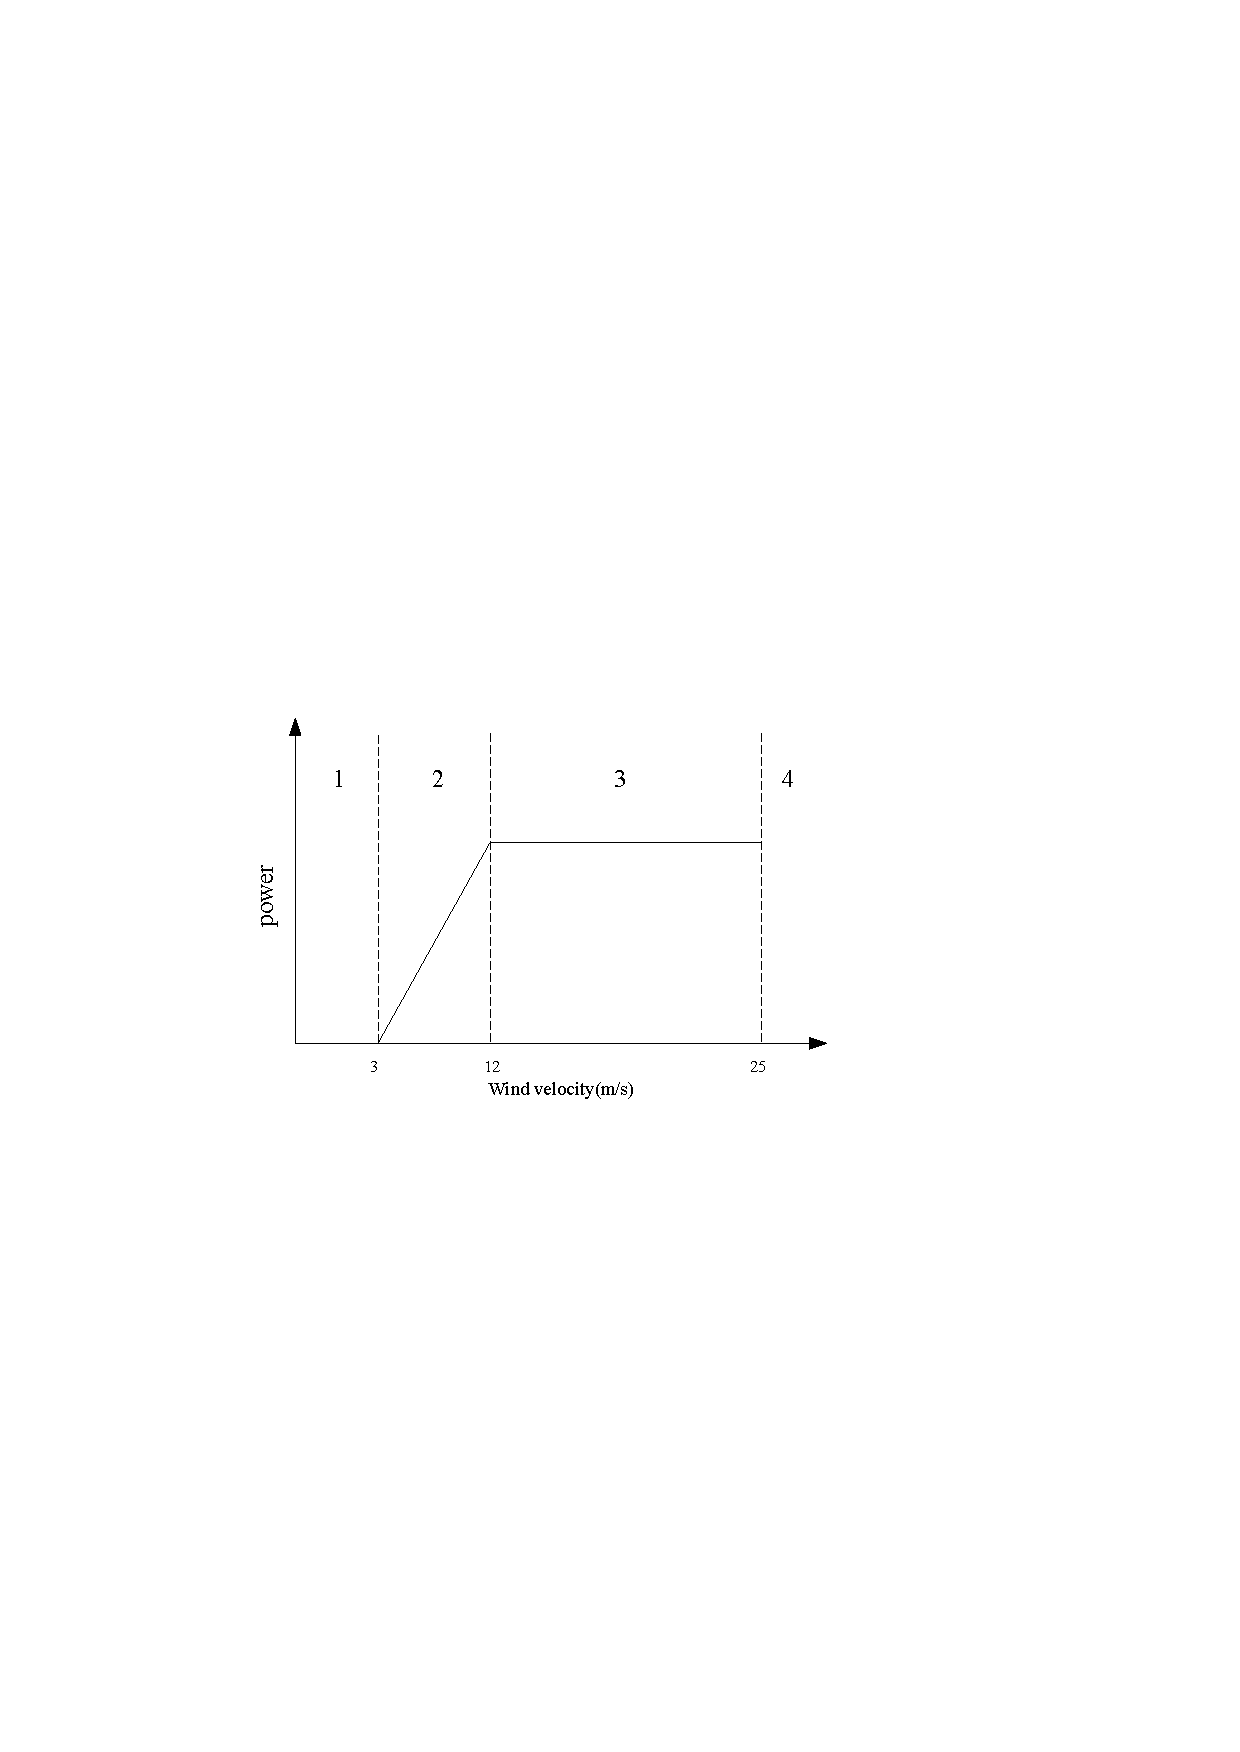
\includegraphics[]{Visio-four_zone.pdf}
  \caption{Four operational zones of wind turbines}
  \label{fig:1}
\end{figure}

The wind turbine operates in four operational zones governed by the mean wind velocity, the four
zones are depicted in Fig. \ref{fig:1}.
In zone 1, the turbine is standstill. In zone 2, the turbine is optimized
to capture the maximum wind power. In zone 3, the pitch system works to keep constant power
production. In zone 4, the wind velocity is too high so that the wind turbine is kept shutdown \cite{ref:wind zone}.
The hydraulic pitch
system fault directly affects the production stability when the
turbine is in zone 3.
The fault diagnosis technology has a wide range of applications in industry. Wang et al. adopt an adaptive
fault diagnosis observer design method combined with the switching technique to estimate the effect
of bias faults and gain faults of the actuator \cite{ref:nody1}.
Xu et al. design a fuzzy state observer to estimate the
faults, which are modeled as both loss of effectiveness and lock-in-place \cite{ref:nody2}.
At present, fault diagnosis
researches of hydraulic variable pitch system for wind turbine are mainly as follows. Wang et al.
have studied to carry on fault diagnosis technology of pressure with integration BP neural network
theory \cite{ref:neural BP}.
% 2013.9.25
Wang's method is effective for the non-linear dynamic process in hydraulic system, but BP
neural network theory still lacks proof and is difficult to obtain the estimation error bound.
% 2013.9.25 remove peti's method, add wavelet method
Goharrizi et al. analyze the pressure signal at one side of the actuator in response to periodic step inputs to the
control valve \cite{ref:qualitative pitch}.
It is shown that with the discrete wavelet transform (WT), the detail information of
pressure signal can be obtained to detect the occurrence of the internal leakage and its severity.
The
similar methods can be found in \cite{ref:hilbert1,ref:hilbert2,ref:hilbert3},
they both use Hilbert Huang transformation method to
process the data, and analyze in the frequency domain. However, the disadvantage is that these method
can only work offline, which limits the use.
%
Sloth et al. use the extended Kalman filter to estimate
the tower acceleration caused by pitch system \cite{ref:active LPV},
by comparing the estimated acceleration value with
true tower acceleration sensor value, Sloth's study is able to determine which pitch is uncontrollable
and the severity of the fault. But Sloth's method relies on the past data, the calculation amount of the
built planning model is increased. This method is also dependent on the tower acceleration sensor,
which is not available in some wind turbines.
% 2013.9.25
%%%%%%%%%
%% 2013.9.24 begin
%%%%%%%%%
% add some description about the disadvantages of conventional diagnosis
%%%%%%%%%
%% 2013.9.25 end
%%%%%%%%%

System identification is one of the major research fields of modern control
theory \cite{ref:ding1}.
A lot of identification methods have been proved
to have minimum estimation error \cite{ref:ding2},
identifiability \cite{ref:ding3}
and be identified online \cite{ref:ding4}.
In this paper, we try to convert the fault diagnosis problem into a system
identification issue. The following faults may happen to pitch system, they
are: pump wear, hydraulic leakage, high air content in the hydraulic
oil \cite{ref:active LPV}.
These faults change the dynamics of the pitch
system and make the system uncontrollable. In system identification view,
the pitch system with fault can be modeled as a time-varying system.
An effective way to estimate the time-varying system is within the framework
of the identification algorithm with a forgetting factor $\lambda$.
%%%%%%%%%
%% 2013.9.25 begin
%%%%%%%%%
% add some description about system identification
%%%%%%%%%
%% 2013.9.25 end
%%%%%%%%%

Some work has been done to deal with the parameter estimation of time-varying system.
In 1995, Guo and Ljung studied the estimation error of recursive least
squares (RLS) with a forgetting factor (RFFLS for short) \cite{ref:rls},
they
assumed that the error $v(t)$ and parameter drift $w(t)$ can be modeled as white
noise. In \cite{ref:rffls,ref:misg},
Ding studied the detail of RFFLS's
estimation error bounds and prove only in deterministic systems, the algorithm
is exponentially convergent.
%
Zeng et al. use the locally weighted
technique to identify the linear parameter varying system. While the data is close to the current time
point, it is given large weight to measurement, while it is far from the current time point, small weight
is given to measurement \cite{ref:lpv}.


The rest of the paper is organized as follows. Section 2 gives the wind turbine model for simulation
and the differential equation model of pitch system. And then a new way is utilized to convert it into
a difference equation model. In Section 3, the algorithm's procedure and analysis of MIFG is given,
which mainly focuses on how to choose the forgetting factor $\lambda$. Section 4 contains a simulation result
and followed by the conclusion in Section 5.


%%%%%%%%%
%% 2013.9.25 begin
%%%%%%%%%
% add wind turbine model
%%%%%%%%%
%% 2013.9.26 end
%%%%%%%%%


\section{The wind turbine model}

It is depicted in Fig. \ref{fig:assembled} that how the sub-models of the wind turbines are connected. The detailed
introduction is described in the Appendix. The system is sampled at a rate of $T = 100Hz$.

\begin{figure}[!htb]
  %\centering
  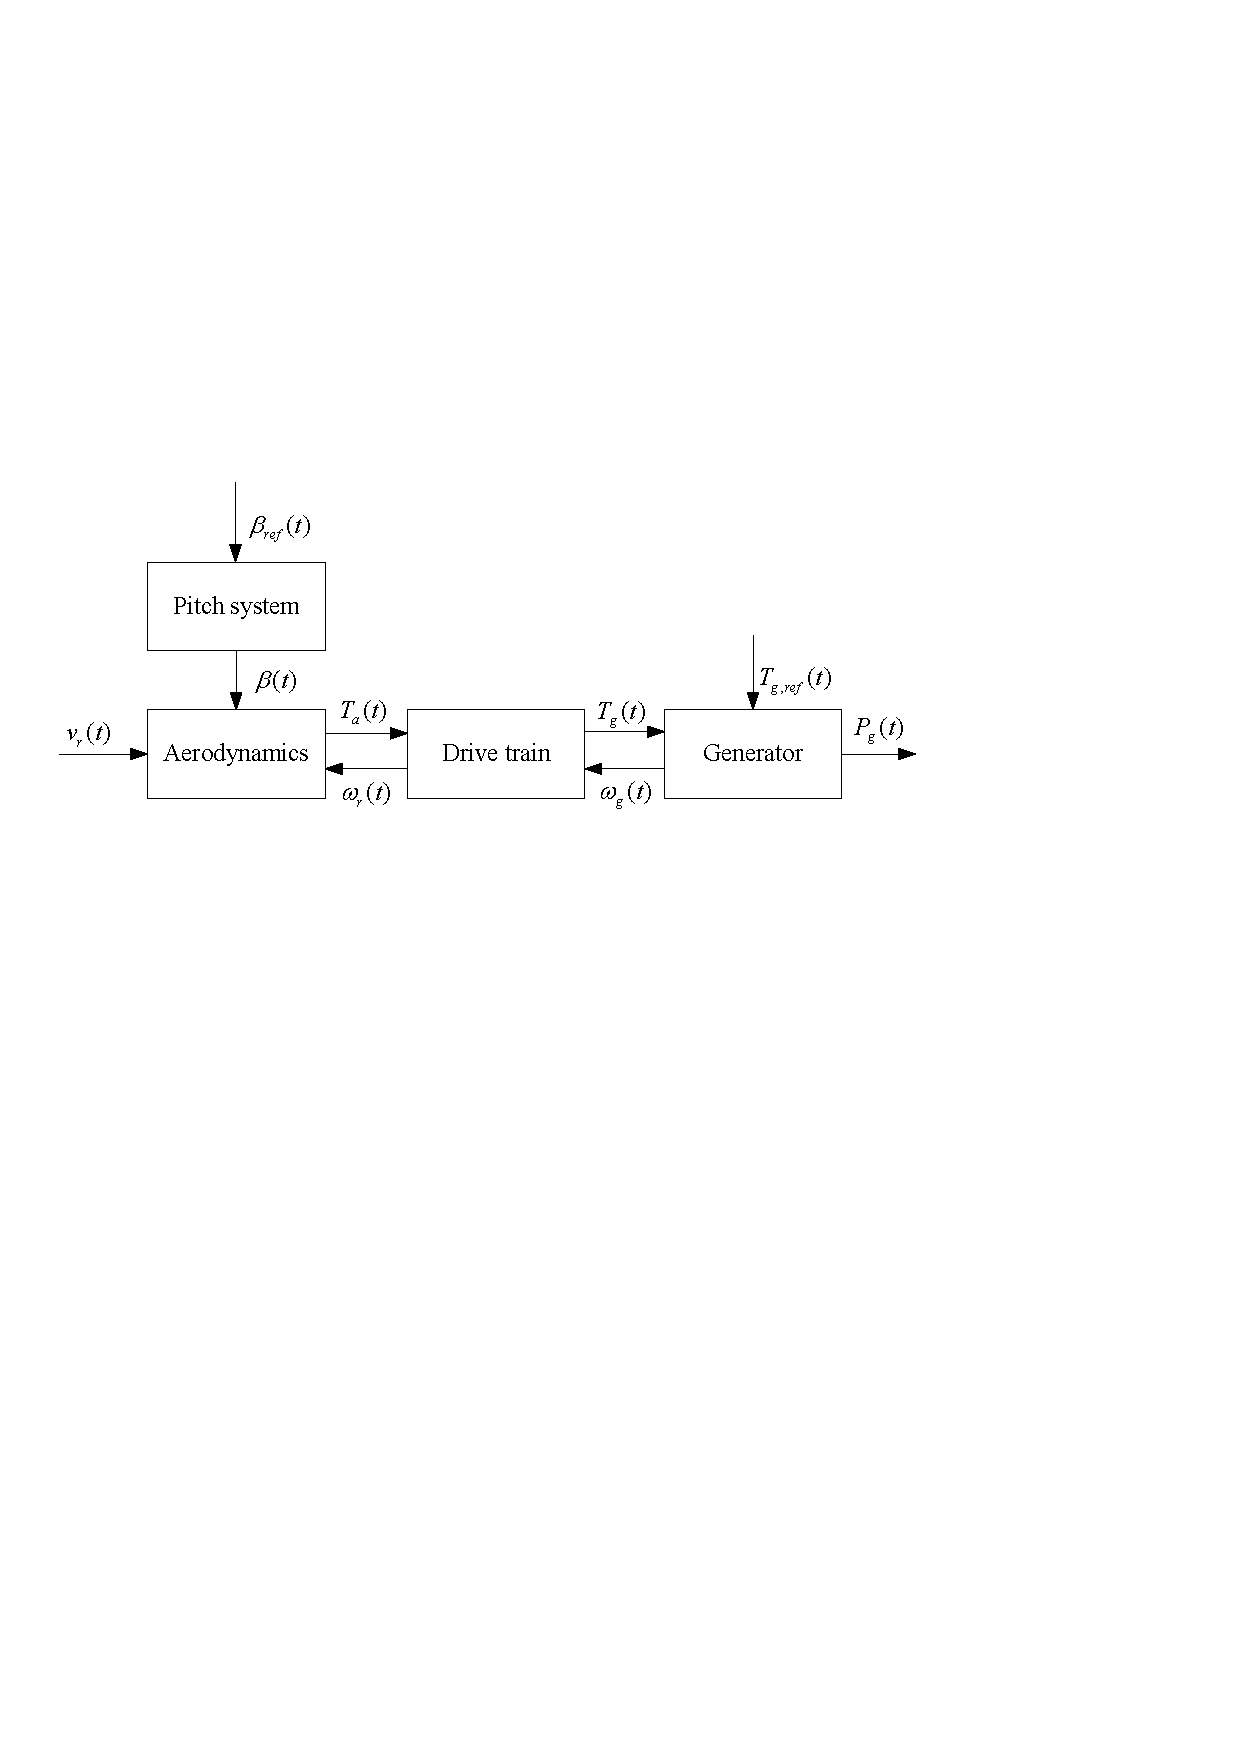
\includegraphics[width=0.8\hsize]{Visio-assembled1.pdf}
  \caption{Structure of the pitch system}
  \label{fig:assembled}
\end{figure}

Since the algorithm will finally be ported to a computer or some embedded processors, it is necessary to change the Eq.(\ref{e:1}) into the difference one. There are many conventional ways to transform the Laplace equation, like bilinear transform and Euler transform, but these methods will lose the accuracy during transformation, and are difficult to meet the industrial requirements.

From the given plant $G(s)$ and sampling period $T$, we can obtain the only linearization model $G(z)$ by applying the impulse invariance transformation method \cite{ref:ding5}.
This method can gurantee the accuracy during transformation from the continuous linear model to the discrete model.

First, we denote
\begin{eqnarray*}
a &:=& -2\zeta\omega_n+\frac{\sqrt{4\zeta^2\omega^2_n-4\omega_n^2}}{2},\\
b &:=& -2\zeta\omega_n-\frac{\sqrt{4\zeta^2\omega^2_n-4\omega_n^2}}{2},\\
G(s) &:=& \frac{\beta(s)}{\beta_{ref}(s)} = \frac{ab}{s^2+(a+b)s+ab},
\end{eqnarray*}
then, by applying the impulse invariance transformation method \cite{DF2013},
the discrete equation is
\begin{eqnarray}
  G(z) &=& \frac{1}{2\pi{}j}\oint_c G(s) \frac{z}{z-e^{Ts}}ds \notag\\
        &=& \frac{1}{2\pi{j}}\oint_c\frac{ab}{(s+a)(s+b)}\frac{1}{1-e^{Ts}z^{-1}}ds \notag \\
        &=& \frac{1}{b-a}\frac{ab(e^{-aT}-e^{-bT})z^{-1}}
        {1 - (e^{-aT}+e^{-bT})z^{-1} + e^{-(a+b)T}z^{-2}} ,
\end{eqnarray}
then, the difference equation can be obtained as
\begin{eqnarray}
  &G(z) = y(t)/u(t) \notag \\
  &(b-a)[1 - (e^{-aT}+e^{-bT})z^{-1} + e^{-(a+b)T}z^{-2}]y(t) \notag \\
  &= [ab(e^{-aT}-e^{-bT})z^{-1}]u(t) ,
\end{eqnarray}
finally,
\begin{eqnarray}
y(t) - (e^{-aT}+e^{-bT})y(t-1) + e^{-(a+b)T}y(t-2) \notag \\
= \frac{ab}{b-a}(e^{-aT}-e^{-bT})u(t-1).
\end{eqnarray}
the identification model can be expressed as
\begin{eqnarray} \label{e:time-varying}
  y(t) = \varphi^\mathrm{T}\theta(t) + v(t),
\end{eqnarray}
where,
$\theta(t):=[- (e^{-aT}+e^{-bT}), e^{-(a+b)T}, \frac{ab}{b-a}(e^{-aT}-e^{-bT})]^\mathrm{T}$, \\ $\varphi(t):=[y(t-1), y(t-2),u(t-1)]^\mathrm{T}$ ,
$v(t)$ is the zero mean white noise.

The faults considered for pitch system are: pump wear, hydraulic leakage, high air content. They can be modeled as
\begin{eqnarray}
  \tilde{\zeta}(t) &=& (1-\alpha_{pw}(t))\zeta + \alpha_{pw}(t)\zeta_{pw} ,\notag \\
  \tilde{\omega}_n(t) &=& (1-\alpha_{pw}(t))\omega_n + \alpha_{pw}(t)\omega_{n,pw}, \\
  \tilde{\zeta}(t) &=& (1-\alpha_{hl}(t))\zeta + \alpha_{hl}(t)\zeta_{hl} ,\notag \\
  \tilde{\omega}_n(t) &=& (1-\alpha_{hl}(t))\omega_n + \alpha_{hl}(t)\omega_{n,hl}, \\
  \tilde{\zeta}(t) &=& (1-\alpha_{ha}(t))\zeta + \alpha_{ha}(t)\zeta_{ha} ,\notag \\
  \tilde{\omega}_n(t) &=& (1-\alpha_{ha}(t))\omega_n + \alpha_{ha}(t)\omega_{n,ha},
\end{eqnarray}
where
$\alpha_{pw}$ is an indicator for the pump wear,
$\alpha_{hl}$ is an indicator for the hydraulic leakage,
$\alpha_{ha}$ is an indicator for the high air content in oil.

The parameters for the above three faults are shown in the table.

\begin{table}[!htb]
  %\centering
  \caption{Parameters' Value}
\begin{tabular}{|c|c|}
  \hline
  % after \\: \hline or \cline{col1-col2} \cline{col3-col4} ...
  Fault & Parameters \\\hline\hline
  No Fault & $\omega_n=11.11rad/s$, \\
            &       $\zeta=0.6$        \\\hline
  Pump Wear & $\omega_{n,pw}=7.27rad/s$,\\
            &       $\zeta_{pw}=0.75$    \\\hline
  Hydraulic Leakage & $\omega_{n,hl}=3.42rad/s$, \\
            &   $\zeta_{n,hl}=0.9$        \\\hline
  High Air Content  & $\omega_{n,ha}=5.73rad/s$, \\
       in the Oil     &   $\zeta_{n,ha}=0.45$ \\
  \hline
\end{tabular}
\end{table}


%%%%%%%%%
%% 2013.9.26 begin
%%%%%%%%%
% add algorithm description
%%%%%%%%%
%% 2013.9.27 end
%%%%%%%%%
\section{The description of fault diagnosis algorithm}

In this section, the procedure to implement the fault diagnosis system is given, and a short discussion is presented on how to choose the forgetting factor $\lambda$ to obtain the minimum estimation error.

\subsection{The structure of the fault diagnosis algorithm}

Fig. \ref{fig:assembled} shows the structure of the wind turbine, the fault diagnosis based on the system identification
theory needs the input data and the output data of the pitch system. We take the pitch controller's
output $\beta_{ref}(t)$ as the input, and the actual pitch angle $\beta(t)$ as the output. The reformed structure is shown below.

\begin{figure}[!htb]
  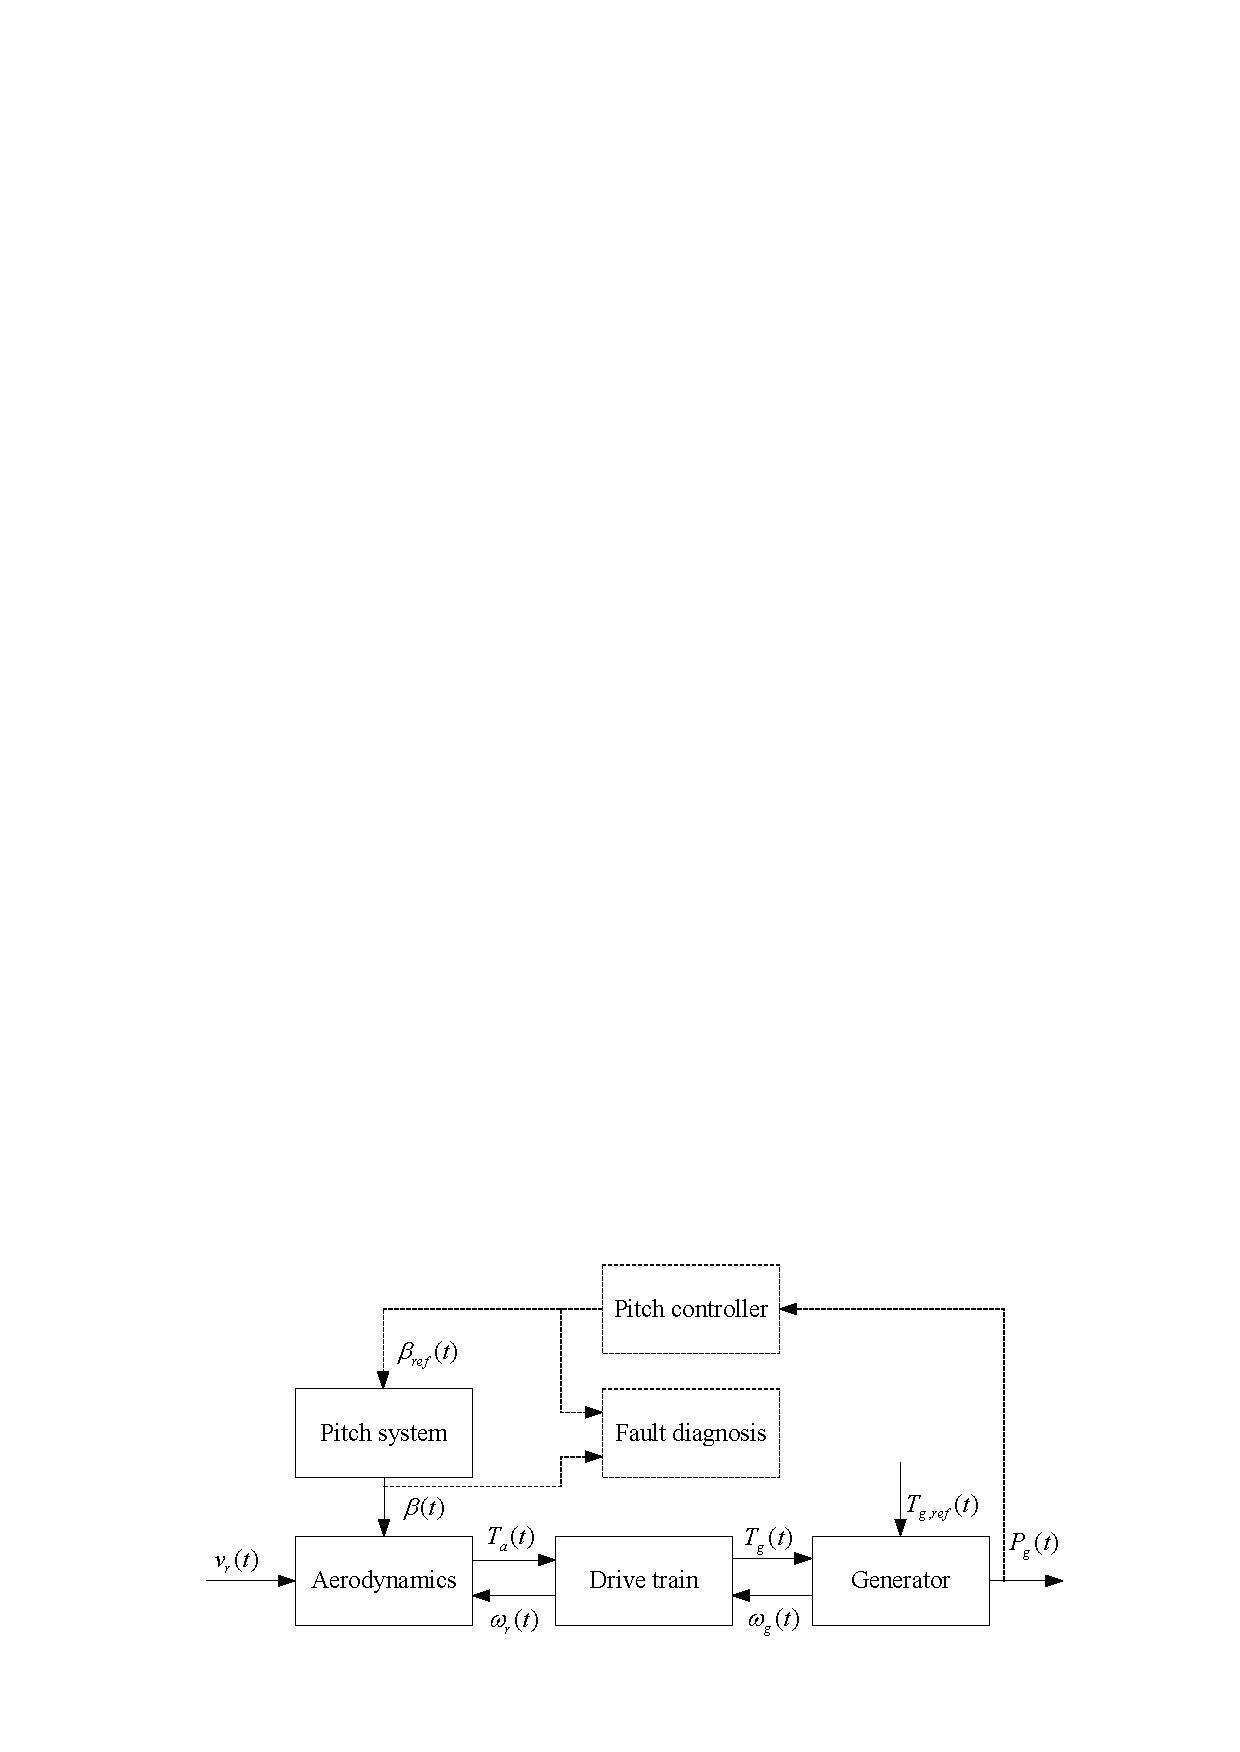
\includegraphics[width=0.8\hsize]{Visio-assembled2.pdf}
  \caption{Simulation structure}
  \label{fig:assembled_diagnosis}
\end{figure}

As the wind turbine in this paper operates in zone 3, the pitch controller is designed by taking the
electric power as the input and pitch reference $\beta_{ref}$ as the output, which will maintain the generated
power constant despite of the disturbance input $v_r(t)$.
%%%%%%%%%
%% 2013.9.26 begin
%%%%%%%%%
% add algorithm description
%%%%%%%%%
%% 2013.9.27 end
%%%%%%%%%

\subsection{The analysis of MIFG}

The innovation is defined as useful information which can improve parameter estimation accuracy \cite{ref:dinf6}. Consider the least square and gradient stochastic algorithms, the identification system is
\begin{equation}
  y(t) = \varphi^\mathrm{T}(t)\theta + v(t),
\end{equation}
where $y(t)\in{}R$ is the output, $\theta(t)\in{}R^n$ is the parameter vector to be identified, $\varphi\in{}R^n$ is the information vector consisting of the system input-output data, $v(t)$ is the stochastic noise with zero mean. The general identification algorithm is
\begin{equation}
  \hat{\theta}(t) = \hat{\theta}(t-1) + L(t)e(t),
\end{equation}
where $L(t)\in{}R^n$ is the gain vector, $e(t):=y(t)-\varphi^\mathrm{T}(t)\hat{\theta}(t-1)\in{}R$ is the scalar innovation, that is the single innovation.

We extend the single innovation to multi-innovation, which means that \\
$E(p,t)=\begin{bmatrix}
  e(t)\\
  e(t-1)\\
  \vdots \\
  e(t-p+1)
\end{bmatrix}\in{}R^p$, $p$ is the innovation length.

By defining the information matrix $\Phi(p,t)$ and stacked output vector $Y(p,t)$ as
$\Phi(p,t)=[\varphi(t),\varphi(t-1),...,\varphi(t-p+1)]\in{}R^{n\times{}p}$,
$Y(p,t)=[y(t),y(t-1),...,y(t-p+1)]^{\mathrm{T}}\in{}R^p$,
the innovation vector $E(p,t)$ may be expressed as
$E(p,t)=Y(p,t) - \Phi^{\mathrm{T}}(p,t)\hat{\theta}(t-1)$.


%%%%%%%%%%%%%%%%%
The faults are reflected in the parameters. When the pitch system operates normally, the identification algorithm is able to figure out the parameter vector. And the parameter of the pitch system
changes correspondingly while the faults happen, the algorithm with a forgetting factor is able to track
the dynamic parameters. So, the MIFG algorithm applied in the pitch system can detect the various
fault situations.

%%%%%%%%%%%%%%%%%

The least square identification algorithm converges fast, but it needs huge computation due to
covariance matrix. The gradient stochastic identification algorithm has a small mount of computation,
but converges slow. Both algorithms are not suitable in wind turbine system. By applying the multi-innovation into the gradient stochastic algorithm, the new algorithm can compute quickly and converge
fast. In order to track a time-varying system, we also apply a forgetting factor $\lambda$, that is MIFG algorithm.

\subsection{How to choose forgetting factor and innovation length}

The purpose of this subsection is to give short discussion on how to choose $\lambda$ and $p$.
Consider the time-varying system Eq.(\ref{e:time-varying}), where $\theta(t)\in{}R^n$ is the time-varying parameter vector to be identified.

The MIFG algorithm of estimating $\theta(t)$ can be expressed as
\begin{eqnarray}
  \hat{\theta}(t) &=& \hat{\theta}(t-1) + \frac{\Phi(t)}{r(t)}[Y(t) - \Phi^\mathrm{T}(t)\theta(t-1)], \label{e:mifg1} \\
  r(t) &=& \lambda{}r(t-1)  + \|\varphi(t)\|^2, 0<\lambda<1, r(0)>0, \label{e:mifg2}
  \\
  \Phi(p,t) &=& [\varphi(t), \varphi(t-1), \ldots, \varphi(t-p+1)]\in{}R^{n\times{}p}, \label{e:mifg3}
  \\
  Y(p,t) &=& [y(t), y(t-1), \ldots, y(t-p+1)]^{\mathrm{T}}\in{}R^p. \label{e:mifg4}
\end{eqnarray}

In engineering, the parameter estimation accuracy is meassured by $\delta_a := \|\hat{\theta}(t) - \theta(t)\|^2$.


The expectation of $E[\|\tilde{\theta}(t)\|^2] $ is  \cite{DF2014}
\begin{eqnarray}
  E[\|\tilde{\theta}(t)\|^2]
  &\leq& [(1+a)(1-\rho)]^t\sigma_0 + \notag
   \frac{3(1+a^{-1})}{1-(1+a)(1-\rho)}[\frac{N^4\beta^2(1-\lambda)^2\sigma^2_w}{2\alpha^2} + \notag
   \frac{N^2\beta(1-\lambda)^2\sigma^2_v}{\alpha^2} + \sigma^2_w]  \label{e:upperbound1}
\end{eqnarray}
and we can denote
\begin{eqnarray}
  [\frac{N^4\beta^2(1-\lambda)^2\sigma^2_w}{2\alpha^2} + \frac{N^2\beta(1-\lambda)^2\sigma^2_v}{\alpha^2} + \sigma^2_w] &:=& f(\lambda) \notag \\
  \frac{3(1+a^{-1})}{1-(1+a)(1-\rho)} &:=& g(a).
\end{eqnarray}
To get the upper bound of the estimation error, we must minimize the right hand side of the Eq.(\ref{e:upperbound1}), let
\begin{equation}
  \frac{dg(a)}{da}=0
\end{equation}
and as we define a to be positive, we can obtain the best value $a_0=\frac{1}{\sqrt{1-\rho}}-1$ ,
and the correspond minimum $g_{min}$ is
$$\frac{3}{(1-\sqrt{1-\rho})^2}$$
and the minimum upper bound can be expressed as
$$[\sqrt{1-\rho}]^t\delta_0 + g_{min}f(\lambda)$$
Since $[\sqrt{1-\rho}]^t\sigma_0$ is very small, we can omit it.  To get the minimum $f_{min}$, just let
\begin{eqnarray}\label{e:f}
  \frac{df(\lambda)}{\lambda}&=&0
\end{eqnarray}
Eq.(\ref{e:f}) is a four-order equation, and generally has four solution to get the best forgetting factor.

From the above analysis, we conclude the following guide to choose the best forgetting factor:
\begin{itemize}
  \item if parameter $\rho$ is small, it will generate small estimation error upper bound, which means $\alpha$ and $\beta$ should be close enough,
  \item the system noise should be as small as possible to get a small estimation error bound,
  \item also from Eq.(\ref{e:f}), a small innovation length $N$ will produce small estimation error upper bound.
\end{itemize}


\section{Simulation}

In this section,  we test the MIFG algorithm in $Matlab/Simulink$ with the model constructed in Section 2 and algorithm described in Section 3. Our identification model is Eq.(\ref{e:time-varying}). The wind turbine operational parameters are shown in the table.

\begin{table}[!htb]
  %\centering
  \caption{Parameter values} \label{tab:turbine parameter}
\begin{tabular}{c|c|c|c}
    \hline
    Parameter        &     Value        &  Parameter     & Value \\ \hline
    $N_g$    & $95$  & $B_r$     & $27.8Nm/(rad/s)$ \\ \hline
    $A$         & $10387m^2$    & $B_{dt}$  & $945kNm/(rad/s)$ \\ \hline
    $\rho$      & $1.225kg/m^3$ & $B_g$     & $3.034Nm/(rad/s)$ \\ \hline
    $J_r$       & $55\times10^6kgm^2$ & $J_g$       & $390kgm^2$  \\ \hline
\end{tabular}
\end{table}

The pitch controller described in Fig. \ref{fig:assembled_diagnosis} is implemented as a PI controller, the detailed simulation structure is shown below. The electric power $P_g$ is the controller input, and the $\beta_{ref}$ is the controller output. Although there is more complex and better controller, but for simulation convenience, we choose the simplest PI controller, where $K_p=4, K_i=1$.

\begin{figure}[!htb]
  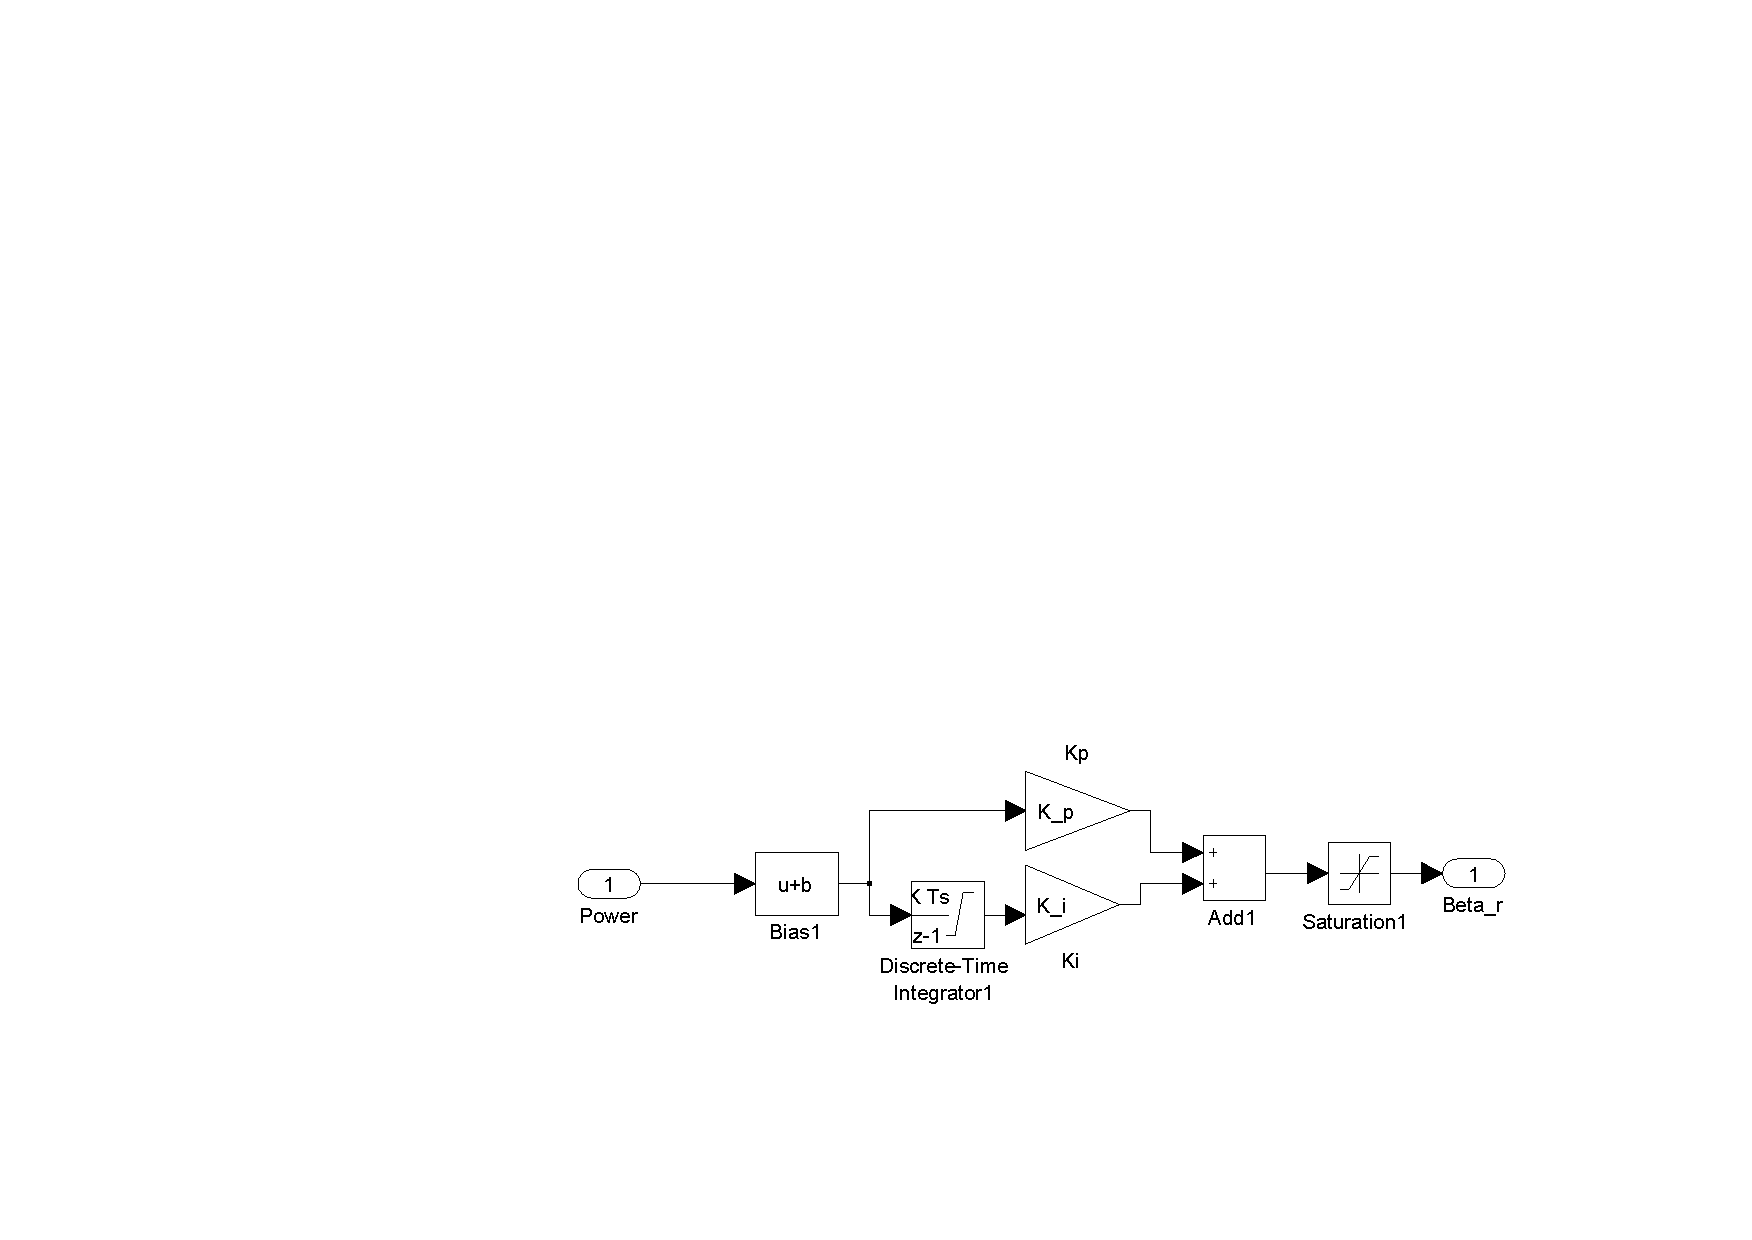
\includegraphics[width=\hsize]{MATLAB_PI.pdf}
  \caption{Simulation model of the PI controller}
  \label{fig:pi_controller}
\end{figure}

The wind data is downloaded from the kk-electronics project, and is depicted in Fig. \ref{fig:wind}. Simulation results are shown in Fig. \ref{fig:pumpwear} to Fig. \ref{fig:highair} where the fault diagnosis result of pump wear fault, hydraulic leakage fault and high air content fault. The forgetting factor is chosen to be $0.97$ according to Eq.(\ref{e:f}), and fault indicator of three situations are the same:

\begin{equation}
  \alpha_{pw},\alpha_{hl},\alpha_{ha}=
  \begin{cases}
    0, & 0\leq{}t\leq1000, 2000\leq{}t\leq3000 \\
    1, & 1000 <t< 2000, 3000 <t< 4500
  \end{cases}
\end{equation}

Results of Fig. \ref{fig:pumpwear} to Fig. \ref{fig:highair} show that when the innovation length gets larger, the algorithm will have a faster convergence. And when the simulation begins, the $p=1$ algorithm fails to track the parameter.


\begin{figure}[!htb]
%\centering
  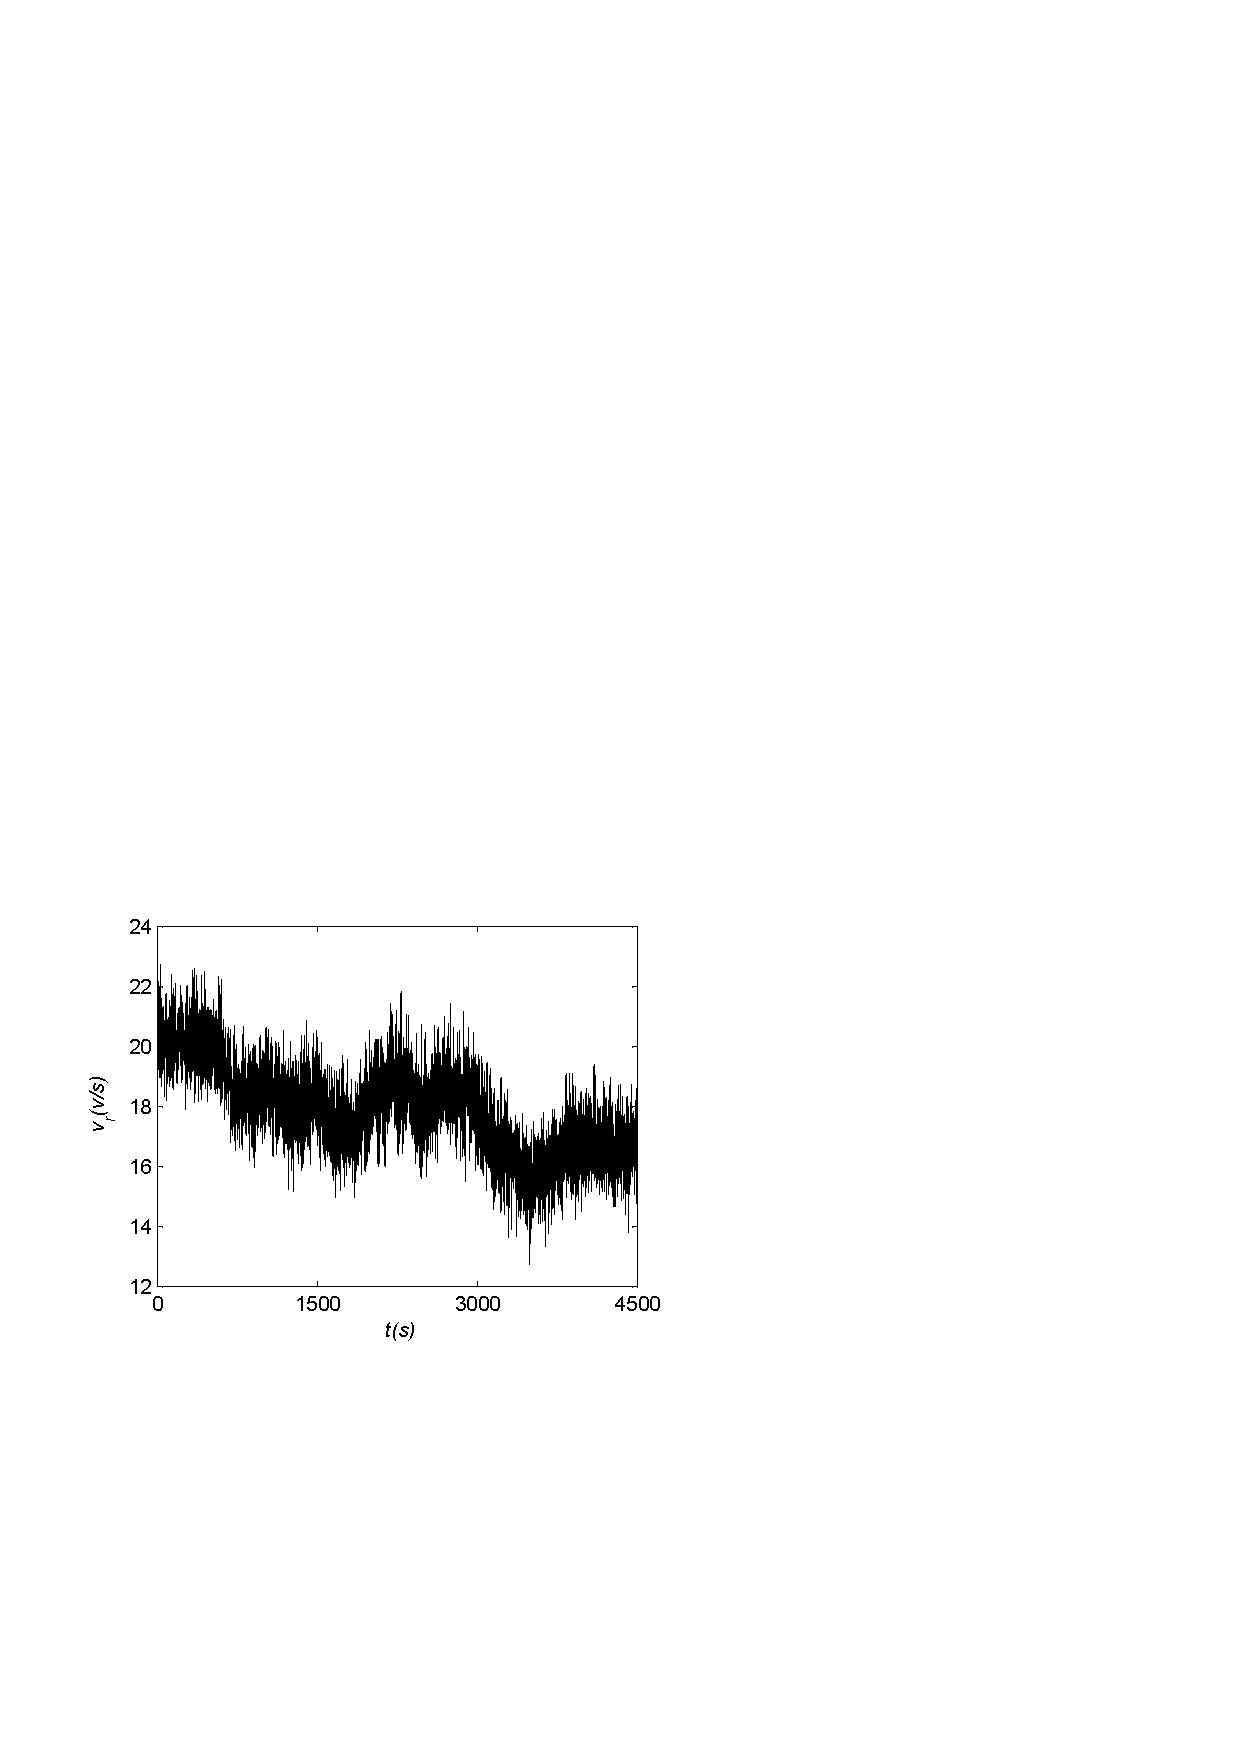
\includegraphics[scale=0.7]{MATLAB_wind.pdf}
  \caption{The wind velocity}
  \label{fig:wind}
\end{figure}
\begin{figure}[!htb]
%\centering
  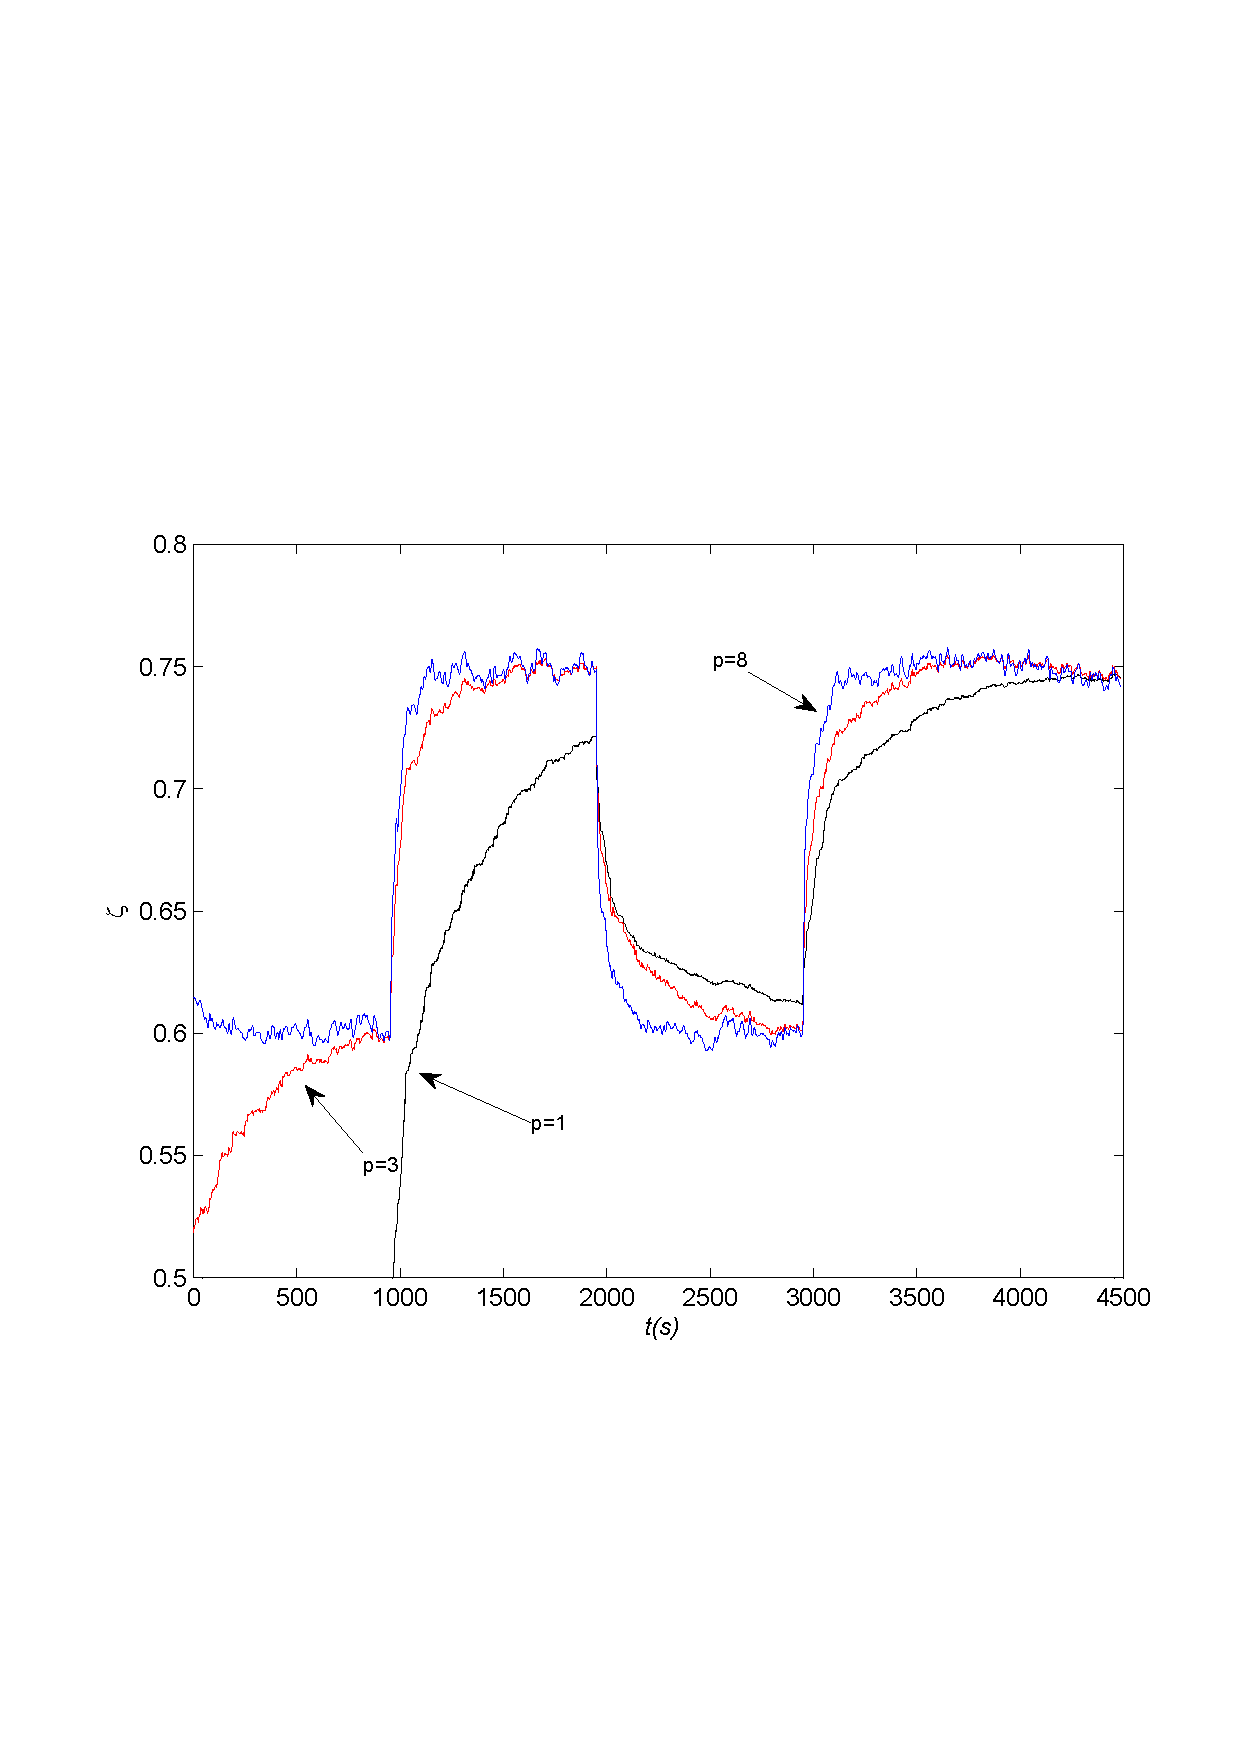
\includegraphics[scale=0.5]{MATLAB_zeta075.pdf}
  \caption{The $\zeta$ with the pump wear fault}
  \label{fig:pumpwear}
\end{figure}
\begin{figure}[!htb]
%\centering
  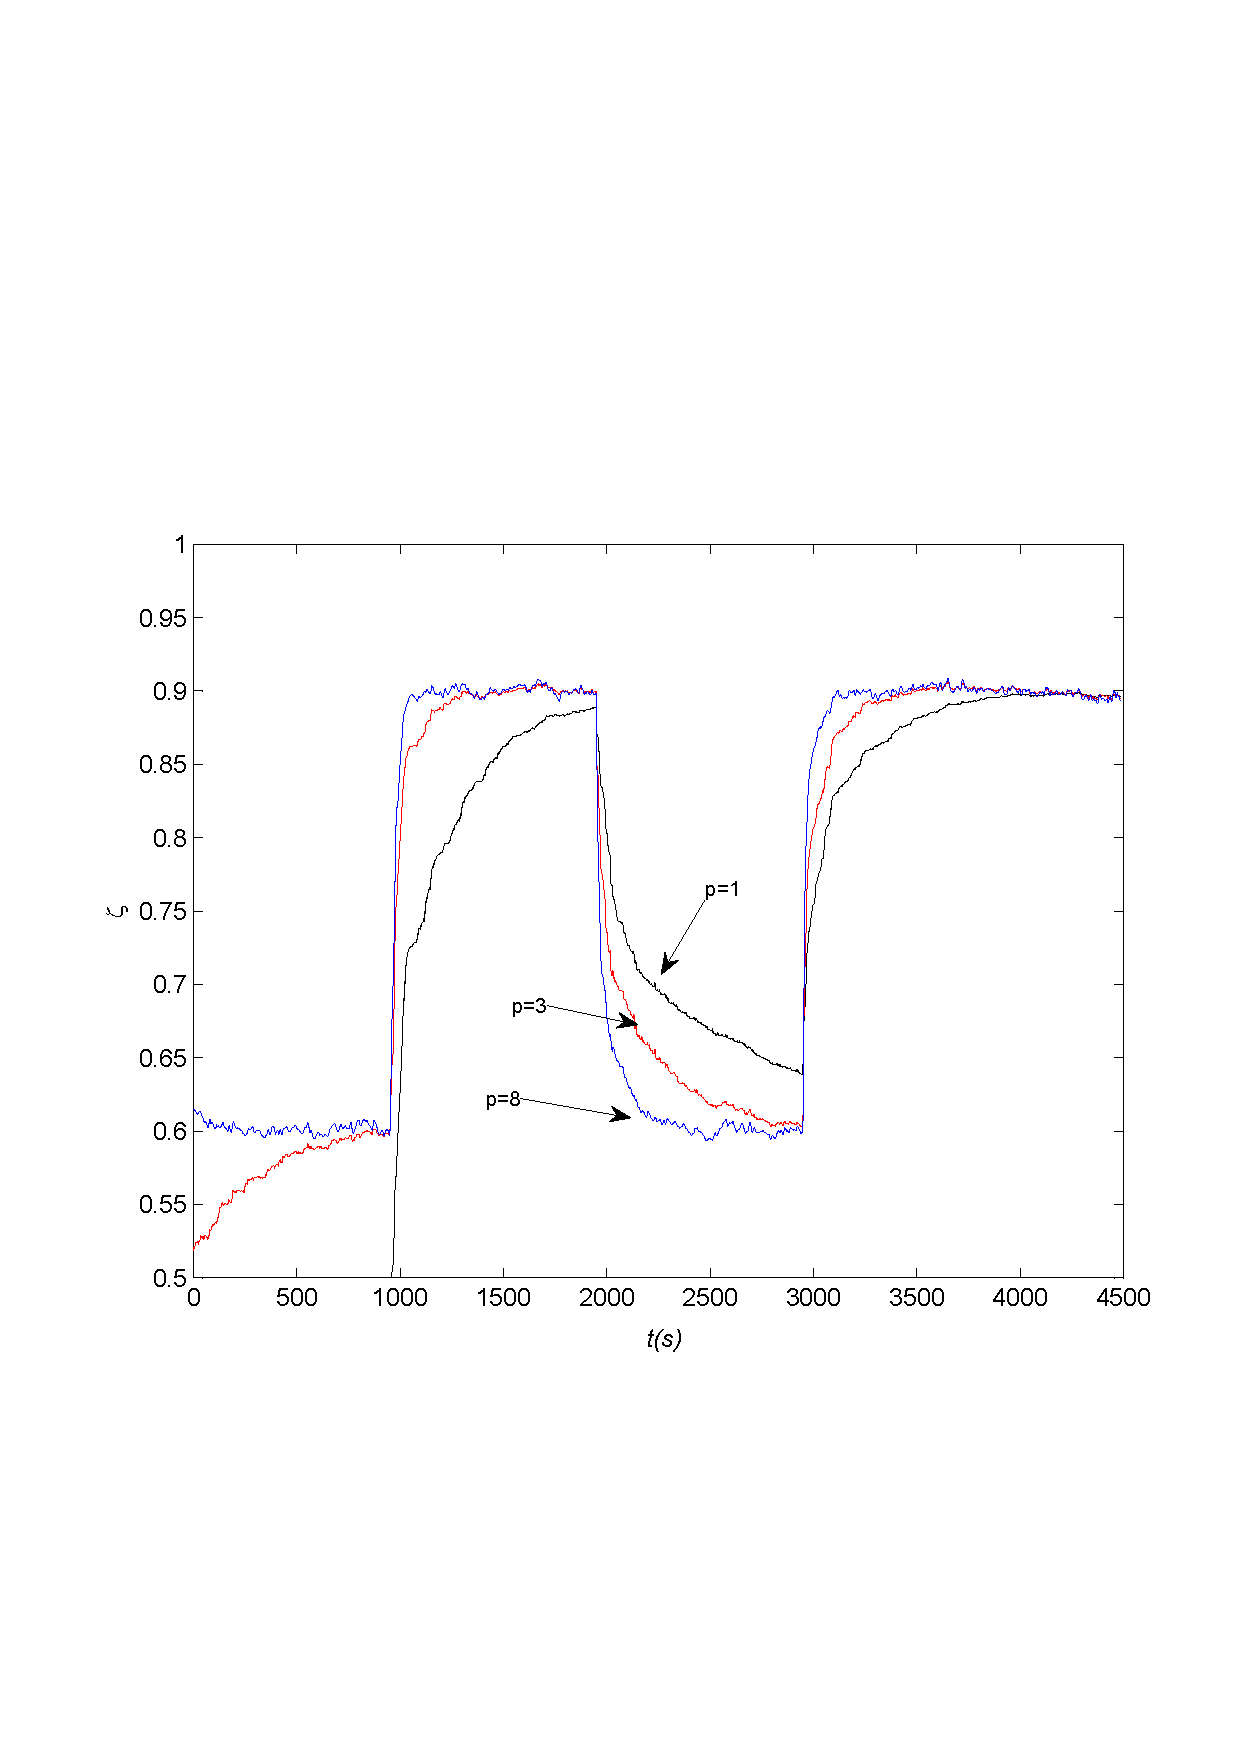
\includegraphics[scale=0.5]{MATLAB_zeta09.pdf}
  \caption{The $\zeta$ with the hydraulic leakage fault}
  \label{fig:leakage}
\end{figure}
\begin{figure}[!htb]
%\centering
  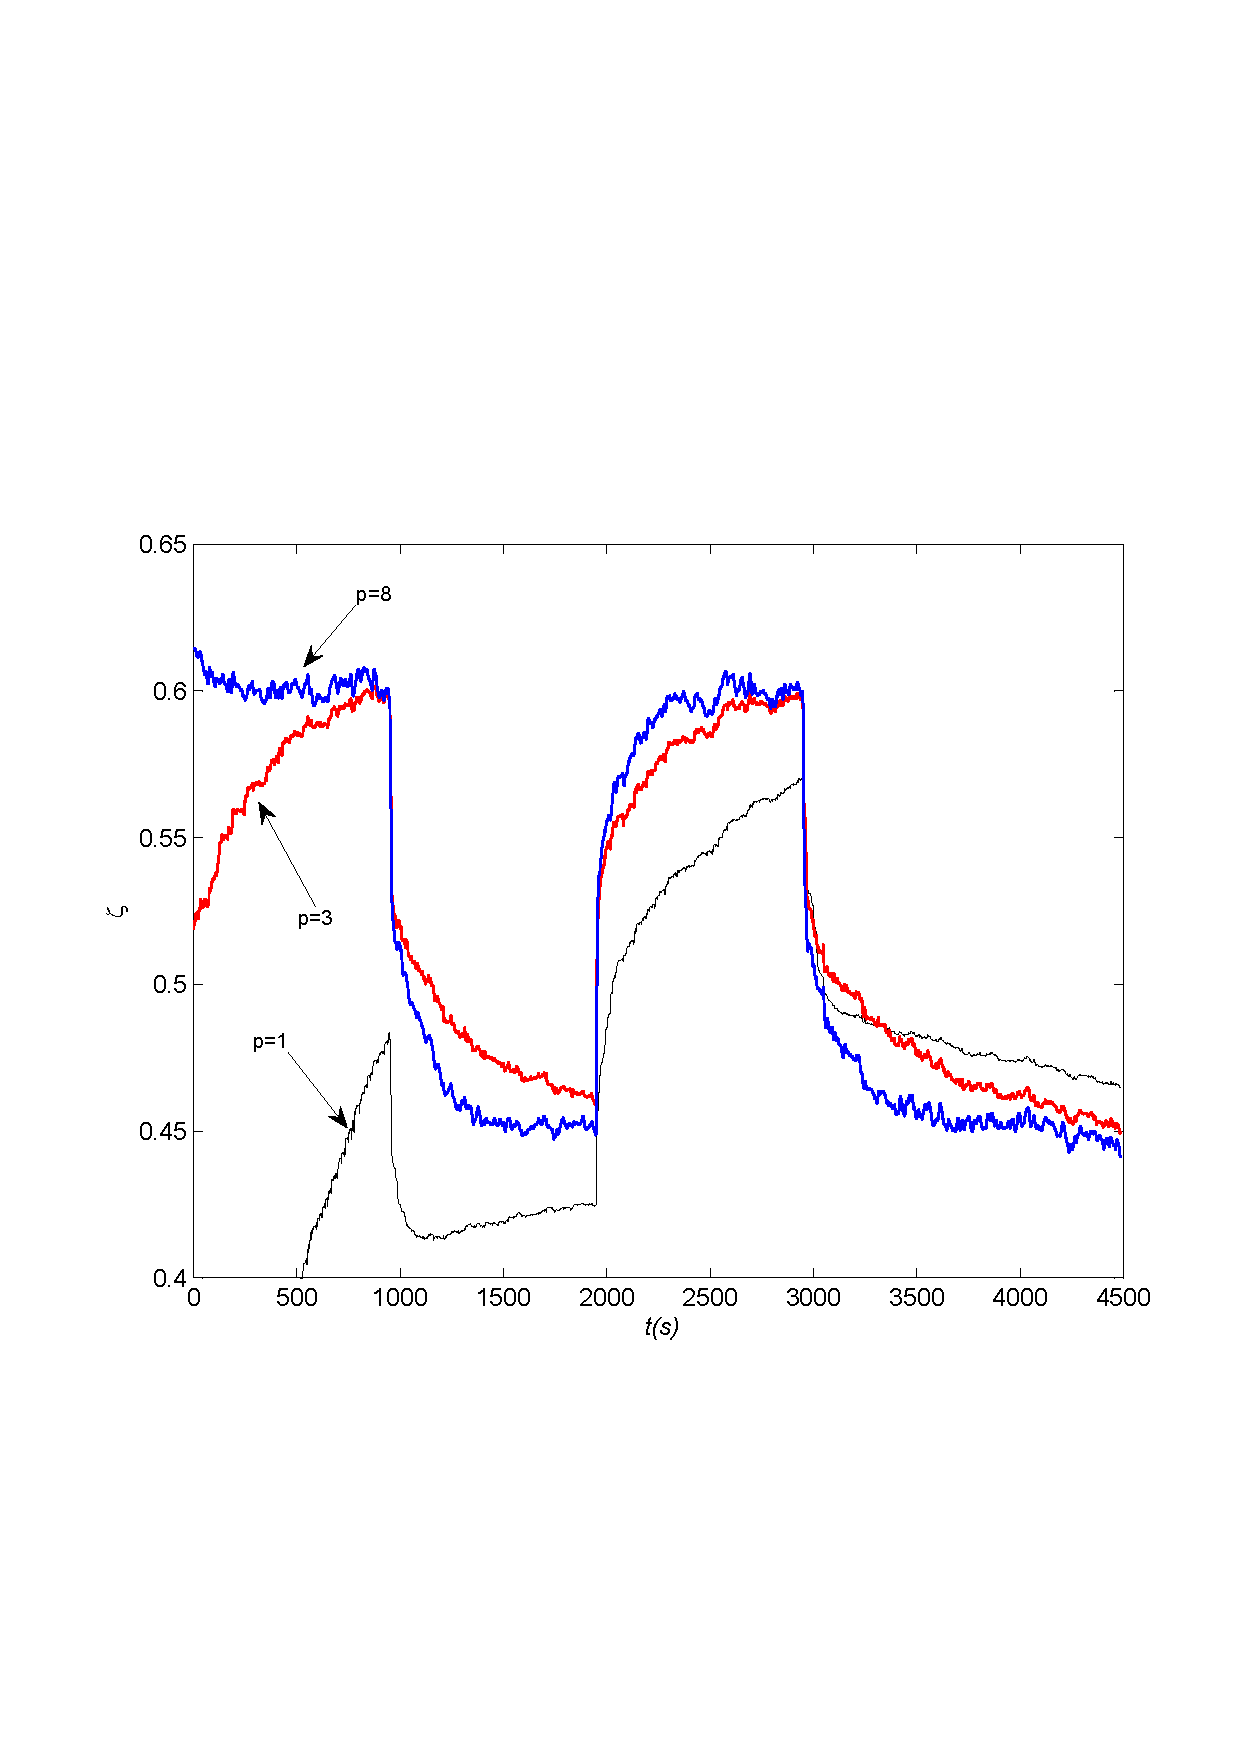
\includegraphics[scale=0.5]{MATLAB_zeta045.pdf}
  \caption{The $\zeta$ with the high air content fault}
  \label{fig:highair}
\end{figure}

We also test the real simulation time, the time is shown in Tab. \ref{tab:time}. As the innovation length gets larger, it takes more computation time as the matrix becomes more complex. As the Tab.\ref{tab:time} suggests, innovation length $p=8$ is better.

\begin{table}[!htb]
  %\centering
  \caption{The real simulation time} \label{tab:time}
\begin{tabular}{|c|c|}
  \hline
  % after \\: \hline or \cline{col1-col2} \cline{col3-col4} ...
  Innovation length & Time \\\hline\hline
    $p=1$     &   $0.313650s$ \\\hline
    $p=3$         & $0.270484s$ \\\hline
    $p=8$         & $0.360650s$ \\\hline
    $p=12$         & $0.497493s$ \\\hline
    $p=14$         & $0.534856s$ \\\hline
    $p=16$         & $0.601536s$ \\\hline
    $p=32$         & $0.894214s$ \\\hline
  \hline
\end{tabular}
\end{table}


\section{Appendix}
In this appendix, we shall give the simulation model of the wind turbine. The turbine is composed
of aerodynamics, pitch, drive train and generator convertor.

The pitch converts the energy from wind to rotor shaft, the shaft rotates at the speed $\omega_r(t)$, the wind power is dependent on wind velocity $v_r(t)$, air density $\rho$ and the rotate area $A$. The converted wind power is based on power coefficient $C_p(\lambda(t), \beta(t))$, where $\lambda(t)$ is tip-speed ratio and $\beta(t)$ is pitch angle. The aerodynamic torque applied on rotor shaft is given as \cite{ref:robust1}

\begin{equation}
  T_a(t) = \frac{1}{2\omega_r(t)}\rho{}Av^3_r(t)C_p(\lambda(t),\beta(t)).
\end{equation}

The drive train is consisted of low-speed shaft and high-speed shaft, the inertias and friction coefficient of both side are $J_r, J_g$ and $B_r, B_g$. The two shafts are interconnected by gears, and the gear ratio is $N_g$, combined with torsion stiffness $K_{dt}$ and torsion damping $B_{dt}$. This results in a torque applied to generator $T_g(t)$ with a speed $\omega_g(t)$. The drive train model is given as\cite{ref:robust2}
\begin{eqnarray}
  J_r\dot{\omega_r}(t) &= T_a(t) + \frac{B_{dt}}{N_g}\omega_g(t)
  & -(B_{dt} + B_r)\omega_r(t), \\
  J_g\dot{\omega_g}(t) &= \frac{B_{dt}}{N_g}\omega_r(t) - T_g(t)
  & -(\frac{B_{dt}}{N^2_g} + B_g)\omega_g(t).
\end{eqnarray}

Electric power is generated by the generator, while the generator torque is adjusted by the reference $T_{g,ref}(t)$. The actual torque from converter is described as a first order system with time constant $\tau_g$ and time delay $t_{g,d}$ \cite{ref:active LPV},
\begin{equation}
  \dot{T_g}(t) = -\frac{1}{\tau_g}T_g(t) + \frac{1}{\tau_g}T_{g,ref}(t-t_{g,d}).
\end{equation}

The electric power produced by the generator is described as follows, where the $\eta$ is efficiency of generator, which is considered to be a constant \cite{ref:active LPV},
\begin{equation}
  P_g(t) = \eta_g\omega_g(t)T_g(t).
\end{equation}
%%%%%%%%%
%% 2013.9.25 begin
%%%%%%%%%
% add wind turbine model
%%%%%%%%%
%% 2013.9.26 end
%%%%%%%%%



The purpose of this section is to explain how the pitch system is modeled. The pitch system shown in Fig.\ref{fig:2} ajusts the pitch of a blade by rotating it according to wind velocity. In general, one turbine is composed of three pitches, each pitch is regulated by a hydraulic actuator, which are controlled separately by three valves.

\begin{figure}[!htb]
  %\centering
  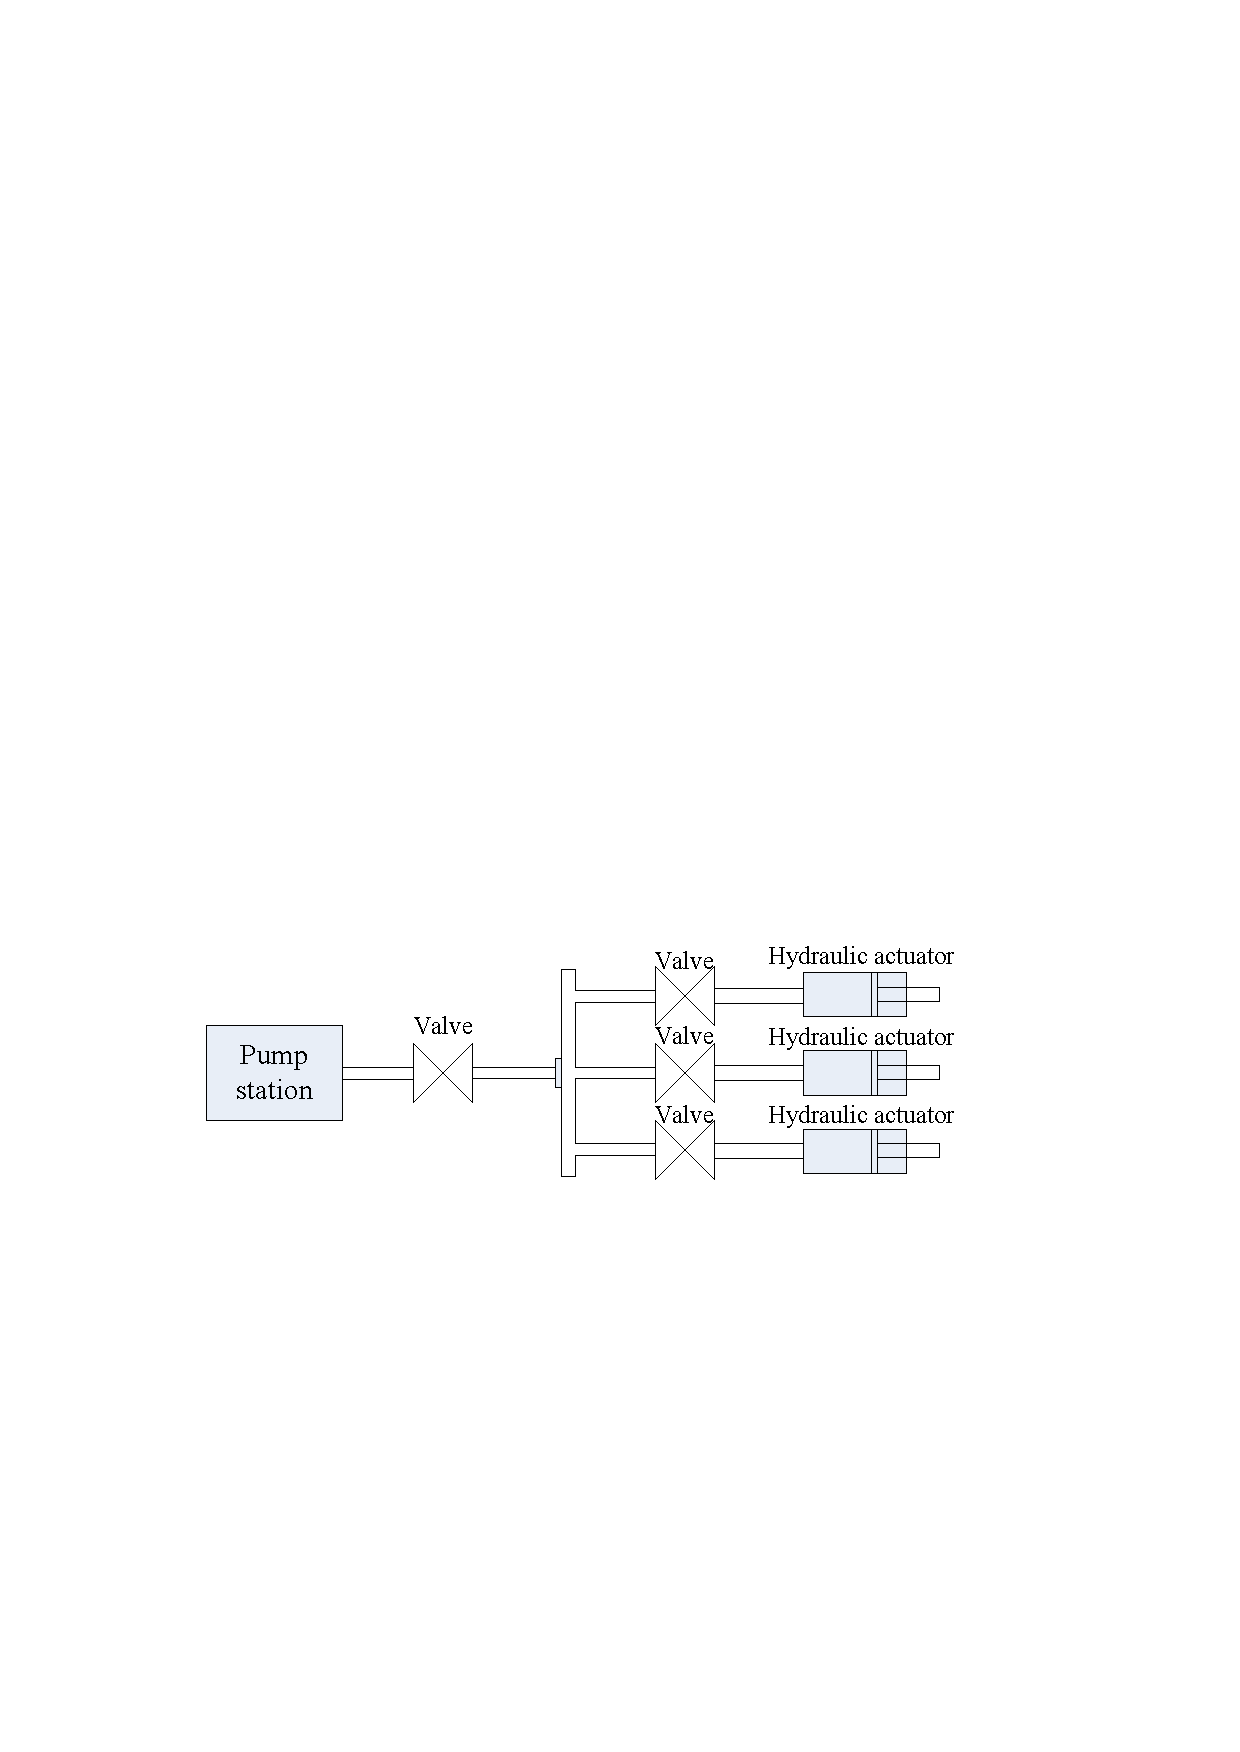
\includegraphics[width=0.8\hsize]{Visio-pitchsystem.pdf}
  \caption{The hydraulic pitch system}
  \label{fig:2}
\end{figure}


The hydraulic pitch is modeled as a second order system,

\begin{eqnarray}\label{e:1}
\frac{\beta(s)}{\beta_{ref}(s)} &=& \frac{\omega^2_n}{s^2 + 2\zeta\omega_n{}s+\omega_n^2} \notag\\
\ddot{\beta}(t) &=& -2\zeta\omega_n\dot{\beta}(t) - \omega^2_n\beta(t) + \omega^2_n\beta(t) + \omega^2_n\beta_{ref}(t),
\end{eqnarray}
where
$\beta(t)$ is the pitch angle,
$\beta_{ref}(t)$ is the reference to the pitch angle,
$\omega_n$ is the natural frequency of the pitch model,
$\zeta$ is the damping ratio of the pitch model.


\footnotesize

\baselineskip 8pt

\begin{thebibliography}{99}



%\bibitem{ref:1}
%Global Wind Energy Council. Global wind report -- annual market
%update 2011. Brussels Belgium: Global Wind Energy Council
%(2012) 1--26.

\bibitem{ref:2}
Dobrila, O., Stefansen, R.: Fault tolerant wind turbine control.
Denmark: Technical  University  of  Denmark (2007) 1-24

\bibitem{ref:3}
Li S.B., Sauter D., Aubrun C.: Stability guaranteed active fault-tolerant control of networked control systems. Journal of Control Science and Engineering. \textbf{2008}(5), 22-31 (2008)

\bibitem{ref:wind zone}
Bianchi F.D., Battista H.D., Mantz R.J.: Wind Turbine Control Systems �C Principle, Modelling and Gain Scheduling Design.
Springer, London (2007)

%%%%%%%%%%%%%%%%%%%%%%5
%%%%%%%%%%%%%%%%%%%%%%
\bibitem{ref:nody1}
Wang H.M., Ye D., Yang G.H.: Actuator fault diagnosis for uncertain TCS fuzzy systems with local
nonlinear models.
Nonlinear Dyn. \textbf{73}(3), 2013-2023 (2013)

\bibitem{ref:nody2}
Xu Y.Y., Tong S.C., Li Y.M.: Adaptive fuzzy fault-tolerant control of static var compensator based
on dynamic surface control technique.
Nonlinear Dyn. \textbf{76}(4), 1977-1988 (2014)
%%%%%%%%%%%%%%%%%%%%%%
%%%%%%%%%%%%%%%%%%%%%%


\bibitem{ref:neural BP}
Wang S.P., Wang Z.L.: The neural network method of hydraulic pump fault
diagnosis. Journal of Beijing University of Aeronautics and
Astronautics.  \textbf{23}(6),  714-718 (1997)

\bibitem{ref:qualitative pitch}
Goharrizi A.Y., Sepehri N.: A wavelet-based approach to internal seal damage diagnosis in hydraulic actuators. IEEE Trans. Ind. Electron. \textbf{57}(5), 1755-1763 (2010)


%%%%%%%%%%%%%%%%%%%%%%5
%%%%%%%%%%%%%%%%%%%%%%
\bibitem{ref:hilbert1}
Roveri N., Carcaterra A.: Damage detection in structures under travelling loads by Hilbert-Huang
transform.
Mech. Sys. Sig. Proc. \textbf{28}(4), 128-144 (2012)

\bibitem{ref:hilbert2}
Feldman M.: Hilbert transform in vibration analysis.
Mech. Sys. and Sig. Proc. \textbf{25}(3), 735-802 (2011)

\bibitem{ref:hilbert3}
Roveri N., Carcaterra A.: Unsupervised identification of damage and load characteristics in time-varying systems. Continuum Mech. Thermodyn. doi: 10.1007/s00161-013-0328-3
%%%%%%%%%%%%%%%%%%%%%%5
%%%%%%%%%%%%%%%%%%%%%%


\bibitem{ref:active LPV}
Esbensen T, Sloth C.
Fault Diagnosis and Fault-Tolerant Control of Wind Turbines.
 Aalborg University.  16-21, 100-104 (2009)

%%%%%%%%%%%%%%%%%%%%%%%
%% 2013.9.27 begin
%%%%%%%%%%%%%%%%%%%%%%%
\bibitem{ref:ding1}
Ljung L.: System identification: Theory for the user. Prentice-Hall: Englewood Cliffs, NJ (1999)

\bibitem{ref:ding2}
Ding F., Chen T.: Modeling and identification for multirate systems. Automatica \textbf{31}(1),  105-122 (2005)

\bibitem{ref:ding3}
Ding F., Lin P., Liu G.: Auxiliary model based multi-innovation extended stochastic gradient parameter estimation with colored measurement noises. Signal Processing \textbf{89}(10),  1883-1890 (2009)

\bibitem{ref:ding4}
Ding F., Chen T.: Hierachical least squares identifiaction methods for multivariable systems. IEEE Trans. Autom. Control \textbf{50}(3),  397-402 (2005)
%%%%%%%%%%%%%%%%%%%%%%%
%% 2013.9.27 end
%%%%%%%%%%%%%%%%%%%%%%%

\bibitem{ref:rls}
Guo L., Ljung L.: Exponential stability of general tracking algorithms. IEEE Trans. Autom. Control  \textbf{40}(8) 1376-1387 (1995)

\bibitem{ref:rffls}
Guo L., Ljung L.: Performance analysis of general tracking algorithms. IEEE Trans. Autom. Control \textbf{40}(8) 1388-1402 (1995)

\bibitem{ref:misg}
Ding F., Chen T.: Performance bounds of forgetting factor least
squares algorithm for time-varying systems with finite measurement data.
IEEE Trans. Cir. Sys. \textbf{52}(3), 555-566 (2005)


%%%%%%%%%%%%%%%%%%
%%%%%%%%%%%%%%%%%%
\bibitem{ref:lpv}
Zeng J.S., Gao C.H., Luo S.H.: Identification of LPV system using locally weighted technique.
Applied Mathematics: A Journal of Chinese Universities. \textbf{25}(4),  411-419 (2010)

%%%%%%%%%%%%%%%%%%
%%%%%%%%%%%%%%%%%%




%%%%%%%%%%%%%%%%%%%%%%%
%% 2013.9.27 begin
%%%%%%%%%%%%%%%%%%%%%%%
%\bibitem{ref:lyy1}
%Spera D.A.: \emph{Wind turbine technology} (1994) 31--42.

\bibitem{ref:robust1}
Muljadi E., Butterfield C.P.: Pitch-controlled variable-speed wind turbine generation. IEEE Trans. Ind. Appl. \textbf{37}(1),  240-246 (2001)

\bibitem{ref:robust2}
Muyeen S.M., Ali M.H., Takahashi R., et al.: Comparative study on transient stability analysis of wind turbine generator system using different drive train models. Renewable Power Generation \textbf{1}(2),  131-141 (2007)

\bibitem{ref:ding5}
Ding F.: System identification. Part B: Basic models for system description. Journal of Nanjing University of Information Science and Technology: Natural Science Edition  \textbf{3}(2), 97-117 (2011)

\bibitem{ref:dinf6}
Ding F., Chen H.B., Li M.: Multi-innvation least squares identification methods based on the auxiliaty model for MISO systems. Appl. Math. Comp. \textbf{187}(2)  658-668 (2007)

% \bibitem{ref:kke}
% kk-electronic a/s. Fault tolerant control of wind turbines a benchmark model.
% http://www.kk-electronic.dk/Default.aspx?ID=9338/(2010).
%%%%%%%%%%%%%%%%%%%%%%%
%% 2013.9.27 end
%%%%%%%%%%%%%%%%%%%%%%%

\bibitem{DF2013} 
Ding F., System Identification -- New Theory and Methods. Science Press, Beijing (2013)
\bibitem{DF2014} 
Ding F., System Identification -- Performances Analysis for Identification Methods. Science Press, Beijing (2014)

\end{thebibliography}

\end{document}
